\documentclass[orange]{simonkoenigzusammenfassung}

\title{Theoretische Informatik 1\\\subtitleformat{Zusammenfassung zum Modul Formale Sprachen und Automatentheorie}}
\author{Simon \textsc{König}}

\usepackage{pgf}
\usepackage{tikz}
\usetikzlibrary{arrows,automata,positioning,trees}

\newcommand{\re}{\mathrm{(r.e.)}}
\newcommand{\rec}{\mathrm{(REC)}}
\newcommand{\csl}{\mathrm{(CSL)}}
\newcommand{\cfl}{\mathrm{(CFL)}}
\newcommand{\dcfl}{\mathrm{(DCFL)}}
\newcommand{\reg}{\mathrm{(REG)}}
\newcommand{\fin}{\mathrm{(FIN)}}

\begin{document}
\maketitle
\tableofcontents

\part{Formale Sprachen und Automatentheorie}
\chapter{Einstieg}
In der Theorie um formale Sprachen geht es grundsätzlich darum, Probleme durch formale Sprachen beschreiben zu können. Diese Probleme werden dann in Klassen eingeordnet und gegeneinander abgregrenzt. Wichtig ist zu verstehen, wie man eine formale Sprache beschreiben kann und wo die Unterschiede zwischen den Klassen liegen.


\input{fsua/alleSprachen.tex}
\chapter{Rekursiv aufzählbare Sprachen}\label{sec:typ0}
\begin{equation*}
	\operatorname{Typ-0} = \re
\end{equation*}



Eine Turingmaschine $M$ \emph{akzeptiert} die Sprache $L$, wenn sie nach endlicher Zeit hält.
Bei Eingaben, die nicht zu $L$ gehören, rechnet sie unendlich lang weiter (dieses Verhalten führt später auf das Halteproblem).
Solche Sprachen $L$ gehören dann zu $\re$, sie sind \emph{semi-entscheidbar}.



\section{Sätze zu $\re$}
\begin{itemize}
	\item Die Klasse der Typ-0 Sprachen ist abgeschlossen unter Sternopertaion, Vereinigung, Schnitt und Konkatenation.
	\item Die Klasse der durch Turingmaschinen erkennbaren/akzeptierten Sprachen ist gleich der Klasse der rekursiv aufzählbaren.
\end{itemize}

\chapter{Entscheidbare Sprachen $\rec$:}
\begin{equation*}
	\rec\subset\re
\end{equation*}

\chapter{Kontextsensitive Sprachen $\csl$: Typ-1}
\begin{equation*}
	\csl\subset\rec\subset\re
\end{equation*}
Wortproblem entscheidbar. Abschluss unter allen Operationen.

\section{Algorithmus zur Entscheidbarkeit des Wortproblems:}
Die Funktion $\mathrm{Abl}_n(X)$ wird iteriert angewendet, bis sich entweder $X$ nicht mehr ändert ($w\not\in L(G)$) oder das gesuchte Wort $w$ in $X$ enthalten ist ($w\in L(G)$).

Dabei ist $n$ die Länge des gesuchten Worts $w$, also $|w|$.

Die Funktion $\mathrm{Abl}_n(X)$ ist für eine Grammatik $G$ wie folgt definiert:
\begin{equation*}
	\mathrm{Abl}_n(X)\coloneqq X\cup\set{w\in(V\cup\Sigma)^\star}{|w|\leq n \wedge \exists y\in X:y\Rightarrow_G w}
\end{equation*}


\section{Automatenmodell LBA:}
Die Kontextsensitiven Sprachen werden von linear beschränkten Automaten akzeptiert.



\section{Beispiele: }
\begin{itemize}
	\item $L_1=\set{a^nb^nc^n}{n\geq 1}$ (drei und mehr gleiche Exponenten)
	\item
\end{itemize}

\chapter{Kontextfreie Sprachen $\cfl$: Typ-2}
\begin{equation*}
	\cfl\subset\csl\subset\rec\subset\re
\end{equation*}
Wort- und Leerheitsproblem entscheidbar.

Beschreib- und erkennbar durch einen nichtdeterministischen Kellerautomaten (PDA).
\section{Automatenmodell PDA:}


\section{Sätze zu den kontextfreien Sprachen:}
\begin{itemize}
	\item Jede kontextfreie Sprache über einem unären Alphabet ist regulär!
	\item Die Klasse der kontextfreien Sprachen ist abgeschlossen unter Sternoperation, Vereinigung und Konkatenation.
	\item Das Wortproblem ($\mathcal O(n^3)$) sowie das Leerheitsproblem sind entscheidbar.
\end{itemize}
\subsection{Pumping-Lemma für Typ-2:}
Sei $L\subseteq \Sigma^\star$ eine kontextfreie Sprache, dann gibt es eine Zahl $n$ so, dass für alle $z\in L$ mit $|z|\geq n$ eine Zerlegung mit $z=uvwxy$ in $u,v,w,x,y\in\Sigma^\star$ exisitert für die die drei Bedingungen erfüllt sind:
\begin{itemize}
	\item $|vx|\geq 1$
	\item $|vwx|\leq n$
	\item $\forall i\in N: uv^iwx^iy\in L$
\end{itemize}


\section{Chomsky-Normalform}
Eine Typ-2 Grammatik $(V,\Sigma,P,S)$ ist in Chomsky-Normalform (CNF),  wenn gilt:
\begin{equation*}
	\forall (u,v)\in P: v\in V^2\cup \Sigma
\end{equation*}
Zu jeder Typ-2 Grammatik existiert eine Grammatik $G'$ in CNF für die gilt $L(G)=L(G')$!
\subsection{Umformungsalgorithmus:}
\begin{enumerate}
	\item Zunächst wollen wir erreichen, dass folgendes gilt: $(u,v)\in P\Rightarrow (|v|>1 \vee v\in \Sigma)$
	\begin{enumerate}
		\item \textbf{Ringableitungen entfernen:}

		Eine Ringableitung liegt vor, wenn es Variablen $A_1,\ldots A_r$ gibt, die sich im Kreis in einander ableiten lassen, d.h. es gibt Regeln $A_i\rightarrow A_{i+1}$ und $A_r\rightarrow A_1$.

		Um dies loszuwerden, werden alle Variablen $A_i$ durch eine neue Variable $A$ ersetzt. Überflüssige Regeln wie $A\rightarrow A$ werden gelöscht.
		\item \textbf{Variablen anordnen:}

		Man legt eine Ordnung der Variablen fest: $V=\simpleset{B_1, B_2, \ldots, B_n}$, hierfür muss gelten:
		\begin{equation*}
			A_i\rightarrow A_j \in P \Leftrightarrow i<j
		\end{equation*}
		Falls dies nicht gilt, müssen Abkürzungen verwendet werden, also alle Produktionen von $A_j$ werden eingesetzt:
		\begin{equation*}
			P=(P\setminus\simpleset{A_i\rightarrow A_j})\cup\set{(A_i,w)}{(A_j,w)\in P}
		\end{equation*}
	\end{enumerate}
	\item Jetzt gilt für jede Regel $(u,v)\in P$ entweder $v\in\Sigma$ oder $|v|\geq 2$.

	Für letztere Regeln werden nun Pseudoterminale eingeführt. Es werden neue Variablen und Produktionen für jedes Terminalsymbol hinzugefügt, z.B. $V_a\rightarrow a$.

	\item \textbf{Letzer Schritt:} Alle rechten Seiten mit $|v|>2$ müssen nun noch auf Länge 2 gekürzt werden. Hierfür werden wiederum neue Variablen eingefügt:%
	\begin{align*}
		A\rightarrow C_1C_2C_3\\
		\intertext{Wird gekürzt zu}
		A\rightarrow C_1D_1\\
		D_1\rightarrow C_2C_3
	\end{align*}
\end{enumerate}

\section{Greibach-Normalform}
Eine Typ-2 Grammatik $(V,\Sigma,P,S)$ ist in Greibach-Normalform (GNF),  wenn gilt:
\begin{equation*}
	\forall (u,v)\in P: v\in \Sigma V^\star
\end{equation*}
Zu jeder Typ-2 Grammatik existiert eine Grammatik $G'$ in GNF für die gilt $L(G)=L(G')$!
\subsection{Umformungsalgorithmus:}
\begin{enumerate}
	\item \textbf{Mh?}

	\item \textbf{Beseitigung von Linksrekursion:}

	Alle Produktionsregeln sind von der Form:
	\begin{align*}
		A&\rightarrow A\alpha_1|\ldots|A\alpha_k|\beta_1|\ldots|\beta_l\\
		\intertext{Diese können durch diese $2k+2l$ Regeln ersetzt werden:}
		A&\rightarrow \beta_1|\ldots|\beta_l\\
		A&\rightarrow \beta_1B|\ldots|\beta_lB\\
		B&\rightarrow \alpha_1|\ldots|\alpha_k\\
		B&\rightarrow \alpha_1B|\ldots|\alpha_kB
	\end{align*}%
	Nun sind keinerlei Linksrekursionen mehr vorhanden!
\end{enumerate}

\section{Beispiele: }
\begin{itemize}
	\item $L_1=\set{a^nb^n}{n\geq 1}$ (zwei gleiche Exponenten)
	\item $L_2=\set{ww^R}{w\in\Sigma^\star}$ (unmarkierte Palindrome)
	\item Korrekt geklammerte arithmetische Ausdrücke (Dyck-Wörter)
\end{itemize}

\chapter{Deterministisch kontextfreie Sprachen}
\begin{equation*}
	\dcfl\subset\cfl\subset\csl\subset\rec\subset\re
\end{equation*}

\section{Automatenmodell DPDA:}\label{dcfl:dpda}
Der deterministische Kellerautomat ist ähnlich definiert wie ein der nichtdeterministische (Siehe \autoref{cfl:pda}).

Der Unterschied zum PDA liegt dabei, dass beim DPDA in jeder Situation nur ein Übergang möglich sein darf,
\begin{equation*}
	\forall z\in Z, a\in\Sigma, A\in\Gamma : |\delta(z,a,A)|+|\delta(z,\epsilon,A)|\leq 1
\end{equation*}
und der DPDA akzeptiert nicht durch leeren Keller sondern durch Endzustände.

\paragraph{Ein deterministischer Kellerautomat ist ein 7-Tupel}
\begin{equation*}
	M=(Z,\Sigma,\Gamma,\delta,z_0,\#, E)
\end{equation*}
\begin{description}
	\item[$Z$] endliche Zustandsmenge
	\item[$\Sigma$] Eingabealphabet
	\item[$\Gamma$] Kelleralphabet
	\item[$\delta$] Überführungsfunktion $\delta:Z\times(\Sigma\cup\simpleset\epsilon)\times\Gamma \rightarrow Z\times\Gamma^\star$
	\item[$z_0$] Startzustand, $z_0\in Z$
	\item[$\#$] Keller-Bottom-Symbol $\#\in \Gamma\setminus\simpleset\Sigma$
	\item[$E$] Endzustandsmenge $E\subseteq Z$
\end{description}

\paragraph{Akzeptierte Sprache eines deterministischen PDA:}
\begin{equation*}
	N(M)\coloneqq\set{w\in \Sigma^\star}{\exists e\in E, V\in \Gamma^\star: (z_0, w, \#)\vdash^\star (e,\epsilon,V)}
\end{equation*}
dies wird auch als \emph{Akzeptieren durch Endzustand} bezeichnet.

Beide Akzeptanzarten, (durch Endzustand und leeren Keller, siehe \autoref{cfl:pda}) sind äquivalent.


\section{Sätze zu $\dcfl$:}
\begin{itemize}
	\item Eine deterministisch kontextfreie Sprache geschnitten mit einer regulären Sprache ist wieder eine deterministisch kontextfreie Sprache.
	\begin{equation*}
		L_1\in\dcfl, L_2\in\reg \Rightarrow L_1\cap L_2\in\dcfl
	\end{equation*}
	\item Die Klasse der deterministisch kontextfreien Sprachen ist nur abgeschlossen unter Komplement.
	\item Das Leerheitsproblem (Markieren von produktiven Variablen), das Wortproblem (in Linearzeit mit Kellerautomat) und das Äquivalenzproblem sind entscheidbar.

	Zum Äquivalenzproblem:
	\begin{align*}
		L=L'&\Leftrightarrow L\subseteq L' \wedge L'\subseteq L\\
				&\Leftrightarrow L\cap \overline{L'} = \emptyset \wedge L'\cap \overline L=\emptyset
	\end{align*}
	entscheidbar, da Abschluss unter Komplement und Leerheitsproblem entscheidbar.
\end{itemize}


\section{Beispiele: }
\begin{itemize}
	\item $L_1=\set{w\$w^R}{w\in\Sigma^\star}$ (markierte Palindrome)
	\item Deterministischer Kellerautomat, der die Sprache $L_2=\set{a^nb^n}{n\geq 1}$ akzeptiert:

	\vspace{1em}
	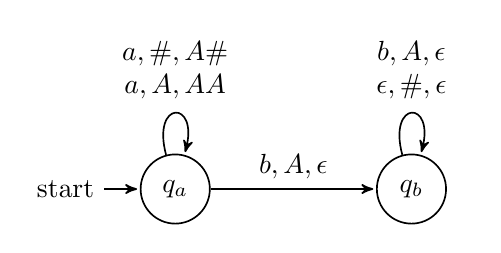
\begin{tikzpicture}[->,>=stealth',shorten >=1pt,auto,node distance=3cm,
	                    semithick]
	  \tikzstyle{every state}=[fill=none,draw=black,text=black]

	  \node[initial,state] 	(A)              {$q_a$};
	  \node[state]         	(B) [right of=A] {$q_b$};

	  \path (A) edge [loop above] node {\begin{tabular}{c}$a,\#,A\#$\\$a,A,AA$ \end{tabular}} (A)
	            edge              node {$b,A,\epsilon$} (B)
	        (B) edge [loop above] node {\begin{tabular}{c}$b,A,\epsilon$\\$\epsilon,\#,\epsilon$ \end{tabular}} (B);
	\end{tikzpicture}

	Konfigurationsübergänge bei Eingabewort $aaabb$:%
	\begin{align*}
		(z_a,aaabb,\#)&\vdash(z_a,aabb,A\#)\\
									&\vdash(z_a,abb,A\#)\\
									&\vdash(z_a,bb,AAA\#)\\
									&\vdash(z_a,b,AA\#)\\
									&\vdash(z_a,\epsilon,A\#)\\
									&\rightsquigarrow aaabb \not\in N(M)=L_2
	\end{align*}
\end{itemize}

\chapter{Reguläre Sprachen}
\begin{equation*}
	\text{Typ-3} = \reg\subset\dcfl\subset\cfl\subset\csl\subset\rec\subset\re
\end{equation*}

\section{Automatenmodell DEA}
Ein deterministischer endlicher Automat ist ein 5-Tupel
\begin{equation*}
	M=(Z,\Sigma,\delta,z_0,E)
\end{equation*}
\begin{description}
	\item[$Z$] endliche Zustandsmenge
	\item[$\Sigma$] Eingabealphabet
	\item[$\delta$] Überführungsfunktion $\delta:Z\times\Sigma\rightarrow Z$
	\item[$z_0$] Startzustand, $z_0\in Z$
	\item[$E$] Endzustandsmenge, $E\subseteq Z$
\end{description}
\bigskip
Es lässt sich außerdem eine erweiterte Funktion $\hat\delta$ definieren:
\begin{align*}
	&\hat\delta:Z\times\Sigma^\star\rightarrow Z\\
	\intertext{Mit den folgenden Eigenschaften:}
	&\hat\delta(z,\epsilon)=z\\
	&\hat\delta(z,ax)=\hat\delta(\delta(z,a),x)
\end{align*}
Die von einem deterministischen Automaten $M$ akzeptierte Sprache ist
\begin{equation*}
	T(M)=\set{w\in\Sigma^\star}{\hat\delta(z_0,w)\in E}
\end{equation*}

\section{Automatenmodell NEA}\label{reg:nea}
Ein nichtdeterministischer endlicher Automat ist ein 5-Tupel
\begin{equation*}
	M=(Z,\Sigma,\delta,S,E)
\end{equation*}
\begin{description}
	\item[$Z$] endliche Zustandsmenge
	\item[$\Sigma$] Eingabealphabet
	\item[$\delta$] Überführungsfunktion $\delta:Z\times\Sigma\rightarrow \Pot(Z)$
	\item[$S$] Startzustandsmenge, $S\subseteq Z$
	\item[$E$] Endzustandsmenge, $E\subseteq Z$
\end{description}
Der NEA ist formal stärker als der DEA, sie akzeptieren jedoch beide die selbe Sprachklasse.

Die akzeptierte Sprache eines nichtdeterministischen endlichen Automaten ist:
\begin{equation*}
	T(M)=\set{w\in\Sigma^\star}{\hat\delta(S,w)\cap E\neq \emptyset}
\end{equation*}

\section{Reguläre Ausdrücke}
Die regulären Sprachen lassen sich zusätzlich zu den zwei Automatenmodellen auch durch sog. reguläre Ausdrücke beschreiben. Eine Definition für die Syntax der regulären Ausdrücke ist:
\begin{itemize}
	\item $\emptyset$ und $\epsilon$ sind reguläre Ausdrücke.
	\item $a$ ist ein regulärer Ausdruck für alle $a\in\Sigma$
	\item Wenn $\alpha$ und $\beta$ eguläre Ausdrücke sind, dann sind auch $\alpha\beta$, $(\alpha|\beta)$ und $(\alpha)^\star$ reguläre Ausdrücke.
\end{itemize}
Die Semantik der regulären Ausdrücke ist ebenso induktiv bestimmt:
\begin{itemize}
	\item $L(\emptyset)=\emptyset$ und $L(\epsilon)=\simpleset{\epsilon}$
	\item $L(a)=\simpleset{a}$ für jedes $a\in\Sigma$
	\item $L(\alpha \beta)=L(\alpha)L(\beta)$, $L(\alpha|\beta)=L(\alpha)\cup L(\beta)$, $L((\alpha)^\star)=L(\alpha)^\star$
\end{itemize}






\section{Sätze zu den regulären Sprachen:}
\begin{itemize}
	\item Typ-3 Sprachen können \emph{nicht} inhärent mehrdeutig sein, da sich zu jeder Sprache ein Minimalautomat bilden lässt.
	\item Die Klasse der Typ-3 Sprachen ist unter allen boole'schen Operationen, Sternoperation und der Konkatenation abgeschlossen.
	\item Für reguläre Sprachen ist das Wortproblem (in Linearzeit), das Leerheitsproblem, das Äquivalenzproblem sowie das Schnittproblem entscheidbar.
	\item Alle Typ-2 Sprachen über einem einelementigen Alphabet sind bereits regulär.
\end{itemize}
\subsection{Pumping-Lemma für Typ-3}%
	Für jede reguläre Sprache $L$ gibt es ein $n\in\N$, so dass für jedes $x\in L$ mit $|x|\geq n$ eine Zerlegung in drei Teile exisitert: $x=uvw$, so dass die drei Bedingungen erfüllt sind:
	\begin{itemize}
		\item $|v|\geq 1$
		\item $|uv|\leq n$
		\item $\forall i \in\N: uv^iw\in L$ (\glqq Pump-Bedingung\grqq)
	\end{itemize}
	\begin{align*}
		\intertext{Gilt die Negation dieser Aussage, also}
		\forall n\in\N:\exists x\in L, |x|\geq n : \forall u,v,w \in\Sigma^\star, x=uvw, |v|\geq 1, |uv|\leq n:\exists i\in\N:uv^iw\not\in L
		\intertext{so ist L nicht regulär!}
 	\end{align*}%

	\textbf{ABER:} Das Pumping-Lemma gibt keine Charakterisierung der Typ-3 Sprachen an! Es gibt auch Sprachen, die nicht Typ-3 sind, die Aussage des Lemmas aber trotzdem erfüllen!

	Das Pumping-Lemma gibt also nur eine Möglichkeit, zu Beweisen, dass eine Sprache \emph{nicht} regulär ist! (Siehe \autoref{bsp:pumpingLemma})
\subsection{Myhill-Nerode-Äquivalenz}%
	Mit der Myhill-Nerode-Äquivalenz ist es möglich nachzuweisen, ob eine Sprache regulär ist.
	\begin{align*}
		&x \mathrm R_L y \Longleftrightarrow \left[\forall w\in\Sigma^\star : xw\in L \Leftrightarrow yw\in L\right]\\
		\intertext{Bzw. anhand eines DEA (dies führt zu einer Verfeinerung von $\mathrm R_L$)}
		&x \mathrm R_M y \Longleftrightarrow \left[\delta (z_0,x)=\delta (z_0,y)\right]\\
		\intertext{Es gilt:}
		&x \mathrm R_M y \Rightarrow \forall w\in\Sigma^\star : \delta (z_0,xw)=\delta (z_0,yw) \Rightarrow x \mathrm R_L y
	\end{align*}
	Die Sprache $L\subseteq \Sigma^\star$ ist genau dann regulär, wenn der Index der Myhill-Nerode-Äquivalenz $\mathrm R_L$endlich ist.


\subsection{Erkennung durch Monoide -- Syntaktisches Monoid}
	Sei $L\subseteq \Sigma^\star$ eine formale Sprache und $M$ ein Monoid.

	$M$ erkennt $L$, wenn eine Teilmenge $A\subseteq M$ und ein Homomorphismus $\varphi:\Sigma^\star \rightarrow M$ existiert, so dass gilt:
	\begin{align*}
		L&=\varphi^{-1}(A) &&\text{d.h. }w\in L \Leftrightarrow \varphi(w)\in A\\
		L&=\varphi^{-1}(\varphi(L)) &&\text{d.h. }w\in L \Leftrightarrow \varphi(w)\in \varphi(L)
	\end{align*}

	Weiter kann man für eine konkrete Sprache $L$ die \emph{syntaktische Kongruenz} definieren:
	\begin{align*}
		w_1\equiv_Lw_2 \Longleftrightarrow [\forall x,y\in\Sigma^\star : xw_1y\in L \Leftrightarrow xw_2y\in L]
	\end{align*}

	Basierend auf dieser Kongruenz definieren wir das Quotientenmonoid der Kongruenz, dessen Elemente die Äquivalenzklassen sind.

	Das Quotientenmonoid oder auch syntaktisches Monoid bezüglich der syntaktischen Kongruenz wird mit
	\begin{equation*}
		\mathrm{Synt}(L)\coloneqq\left(\Sigma^\star/\equiv_L\right)
	\end{equation*}
	bezeichnet.

	Für jede Sprache $L$ gibt es ein syntaktisches Monoid das $L$ mit dem Homomorphismus
	\begin{equation*}
		\varphi: L\rightarrow \mathrm{Synt}(L), w\mapsto [w]
	\end{equation*}
	erkennt.
	Ist $|\mathrm{Synt}(L)|$ endlich, so ist $L$ regulär bzw. erkennbar.

	\subsection{Wohldefiniertheit des Produkts der Äquivalenzklassen}
	\begin{equation*}
		[u_1]_{\equiv_L}*[u_2]_{\equiv_L}\overset ? = [u_1u_2]_{\equiv_L} \quad\text{wohldefiniert?}
	\end{equation*}

	Es gilt:
	\begin{align}
		u_1,\widetilde{u_1}\in[u_1]_{\equiv_L} \Longleftrightarrow u_1\equiv_L \widetilde{u_1} \Longleftrightarrow \left[\forall x,y\in\Sigma^\star : xu_1y\in L \Leftrightarrow x\widetilde{u_1}y\in L\right]\label{reg:produktaequi1}\\
		u_2,\widetilde{u_2}\in[u_2]_{\equiv_L} \Longleftrightarrow u_2\equiv_L \widetilde{u_2} \Longleftrightarrow \left[\forall x,y\in\Sigma^\star : xu_2y\in L \Leftrightarrow x\widetilde{u_2}y\in L\right]\label{reg:produktaequi2}
	\end{align}
	\begin{align*}
		\intertext{Setzt man nun in \autoref{reg:produktaequi1} für $y=u_2y'$ ein:}
		&u_1,\widetilde{u_1}\in[u_1]_{\equiv_L} \Longleftrightarrow u_1\equiv_L \widetilde{u_1} \Longleftrightarrow \left[\forall x,y'\in\Sigma^\star : xu_1u_2y'\in L \Leftrightarrow x\widetilde{u_1}u_2y'\in L\right]\\
		\intertext{Äquivalent gilt das selbe für $\widetilde{u_2}$. Ebenso gilt das gleiche für \autoref{reg:produktaequi2} mit $x=x'u_1$:}
		&u_2,\widetilde{u_2}\in[u_2]_{\equiv_L} \Longleftrightarrow u_2\equiv_L \widetilde{u_2} \Longleftrightarrow \left[\forall x',y\in\Sigma^\star : x'u_1u_2y\in L \Leftrightarrow x'u_1\widetilde{u_2}y\in L\right]
		\intertext{Äquivalent gilt das selbe für $\widetilde{u_1}$. Setzt man nun alle Gleichungen zusammen, erhält man:}
		&u_1u_2\equiv_L \widetilde{u_1}\widetilde{u_2} \Longleftrightarrow \left[\forall x,y\in\Sigma^\star : xu_1u_2y\in L \Leftrightarrow x\widetilde{u_1}\widetilde{u_2}y\in L\right]\\
		\intertext{Dies gilt wie oben gezeigt für alle Kombinationen $u_1u_2, u_1\widetilde{u_2}, \widetilde{u_1}u_2$ und $\widetilde{u_1}\widetilde{u_2}$. Damit erzeugt diese Äquivalenz die Klasse:}
		&[u_1u_2]_{\equiv_L} \text{ mit } u_1u_2, u_1\widetilde{u_2}, \widetilde{u_1}u_2,\widetilde{u_1}\widetilde{u_2}\in[u_1u_2]_{\equiv_L}
	\end{align*}



\section{Beispiele: }
\begin{itemize}
	\item $L_1=\Sigma^\star$
	\item $L_2=L\left((a|b)a(a|b)a^\star\right)$

	\vspace{1em}
	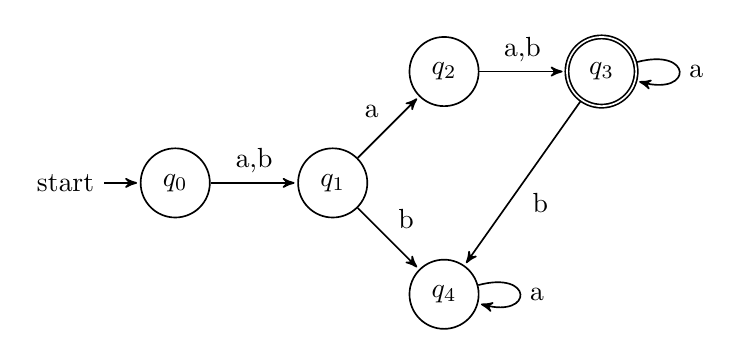
\begin{tikzpicture}[->,>=stealth',shorten >=1pt,auto,node distance=2cm,
	                    semithick]
	  \tikzstyle{every state}=[fill=none,draw=black,text=black]

	  \node[initial,state] (A)              {$q_0$};
	  \node[state]         (B) [right of=A] {$q_1$};
	  \node[state]         (C) [above right of=B] {$q_2$};
		\node[state, accepting] (D) [right of=C] {$q_3$};
		\node[state]         (E) [below right of=B] {$q_4$};

		\path (A) 	edge node {a,b} (B)
					(B)				edge node {a} (C)
	            			edge node {b} (E)
					(C) 			edge node {a,b} (D)
					(D) 		edge [loop right] node {a} (D)
	            			edge node {b} (E)
					(E)				edge [loop right] node {a} (E);
	\end{tikzpicture}
	\item Automat $M$ mit $L_3=T(M)=\set{(ab)^n}{n\in\N_0}$:\\

	\vspace{1em}
	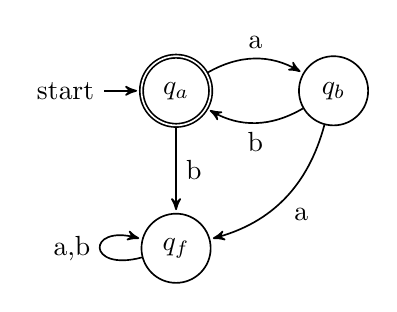
\begin{tikzpicture}[->,>=stealth',shorten >=1pt,auto,node distance=2cm,
	                    semithick]
	  \tikzstyle{every state}=[fill=none,draw=black,text=black]

	  \node[initial,state,accepting] (A)                    {$q_a$};
	  \node[state]         (B) [right of=A] {$q_b$};
	  \node[state]         (C) [below of=A] {$q_f$};

	  \path (A) edge [bend left]  node {a} (B)
	            edge              node {b} (C)
	        (B) edge [bend left]  node {b} (A)
	            edge [bend left]  node {a} (C)
	        (C) edge [loop left]  node {a,b} (C);
	\end{tikzpicture}

	\item Automat erkennt die Sprache

	$L_3=\set{w\in\simpleset{a,b,c}^\star}{w \text{ enthält das Teilwort $abc$ aber nicht das Teilwort $ab$}}$:

	\vspace{1em}
	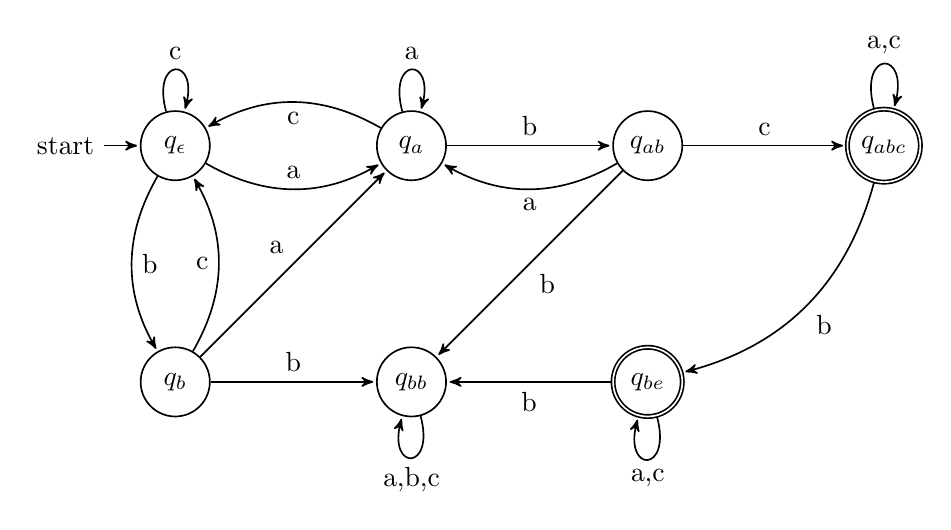
\begin{tikzpicture}[->,>=stealth',shorten >=1pt,auto,node distance=3cm,
	                    semithick]
	  \tikzstyle{every state}=[fill=none,draw=black,text=black]

	  \node[initial,state]   (Epsilon)   {$q_\epsilon$};
	  \node[state]           (A) [right of=Epsilon] {$q_a$};
	  \node[state]           (AB) [right of=A] {$q_{ab}$};
		\node[state, accepting](ABC) [right of=AB] {$q_{abc}$};
		\node[state]           (B) [below of=Epsilon] {$q_b$};
		\node[state]           (BB) [right of=B] {$q_{bb}$};
		\node[state, accepting](BE) [right of=BB] {$q_{be}$};

	  \path (Epsilon) edge [loop above] node {c} (Epsilon)
	            			edge [bend right] node {a} (A)
										edge [bend right] node {b} (B)
					(A)				edge [loop above] node {a} (A)
	            			edge              node {b} (AB)
										edge [bend right] node {c} (Epsilon)
					(AB) 			edge [bend left]  node {a} (A)
	            			edge              node {b} (BB)
										edge              node {c} (ABC)
					(ABC) 		edge [loop above] node {a,c} (ABC)
	            			edge [bend left]  node {b} (BE)
					(B)				edge              node {a} (A)
										edge              node {b} (BB)
										edge [bend right] node {c} (Epsilon)
					(BB)			edge [loop below] node {a,b,c} (BB)
					(BE)			edge [loop below] node {a,c} (ABC)
										edge              node {b} (BB);
	\end{tikzpicture}
\end{itemize}

\chapter{Endliche Sprachen}
\begin{equation*}
	\fin\subset\reg\subset\dcfl\subset\cfl\subset\csl\subset\rec\subset\re
\end{equation*}
Alle endlichen Sprachen sind regulär.

\section{Beispiele}
\begin{itemize}
	\item $L_1=\emptyset$ (leere Sprache ist endlich)
	\item $L_2=\Sigma$ (nur die Buchstaben)
	\item $L_3=\simpleset{aaa,baba}$ (z.B. nur zwei Wörter)
\end{itemize}

\chapter{Algorithmen}
\section{Konstruktionsalgorithmus für Minimal-DEAs:}
Mit dem Beweis zur Myhill-Nerode-Äquivalenz wird ein Automat definiert, dieser ist isomorph zum Minimalautomaten.
Der Index der Myhill-Nerode-Äquivalenz ist genau die Anzahl der Zustände des Minimalautomaten.

Man kann mit einem einfachen Algorithmus aus einem beliebigen DEA den Minimalautomaten erzeugen:

Wir ermitteln algorithmisch, welche Zustände nicht äquivalent sind und verschmelzen die übrig bleibenden.
Nicht äquivalent sind Zustände, bei denen bei Eingabe eines Worts vom einen aus ein Endzustand erreicht wird, vom anderen jedoch nicht.

So sind im ersten Schritt Zustandspaare aus Endzustand und Nichtendzustand nicht äquivalent und werden markiert.

\subsection*{Am Beispiel:}

\vspace{1em}
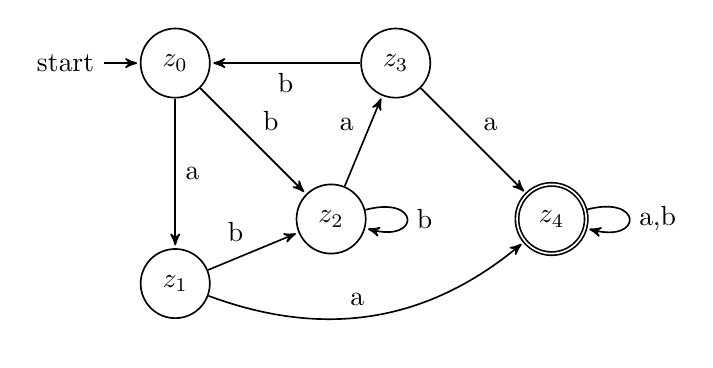
\begin{tikzpicture}[->,>=stealth',shorten >=1pt,auto,node distance=2.8cm,
										semithick]
	\tikzstyle{every state}=[fill=none,draw=black,text=black]

	\node[initial,state] 						(A)              {$z_0$};
	\node[state]         						(B) [below of=A] {$z_1$};
	\node[state]         						(C) [below right of=A] {$z_2$};
	\node[state]         						(D) [right of=A] {$z_3$};
	\node[state, accepting]         (E) [right of=C] {$z_4$};

	\path (A) edge 							node {a} (B)
						edge			  			node {b} (C)
				(B) edge [bend right] node {a} (E)
						edge 						  node {b} (C)
				(C) edge 						  node {a} (D)
						edge [loop right] node {b} (C)
				(D) edge 						  node {a} (E)
						edge 							node {b} (A)
				(E) edge [loop right] node {a,b} (E);
\end{tikzpicture}


Die Paare $\simpleset{z_i,z_4}$ mit $i=0,1,2,3$ werden markiert:

\begin{tabular}{ccccc}
	\cline{2-2}
	$z_1$ & 	\multicolumn{1}{|c|}{ }		&				&				&			 \\
	\cline{2-3}
	$z_2$ & 	\multicolumn{1}{|c|}{ }		&		\multicolumn{1}{c|}{ }		&				&			 \\
	\cline{2-4}
	$z_3$ & 	\multicolumn{1}{|c|}{ }		&		\multicolumn{1}{c|}{ }		&		\multicolumn{1}{c|}{ }		&			 \\
	\cline{2-5}
	$z_4$ & 	\multicolumn{1}{|c|}{$\epsilon$}		&		\multicolumn{1}{c|}{$\epsilon$}		&		\multicolumn{1}{c|}{$\epsilon$}		&		\multicolumn{1}{c|}{$\epsilon$}	 \\
	\cline{2-5}
				& $z_0$ & $z_1$ & $z_2$ & $z_3$\\
\end{tabular}

Durch Testen der Zustandspaare erhält man die untenstehende Tabelle. Hierbei wurden Zeugen für die Antivalenz eingetragen.

\begin{tabular}{ccccc}
	\cline{2-2}
	$z_1$ & 	\multicolumn{1}{|c|}{a}		&				&				&			 \\
	\cline{2-3}
	$z_2$ & 	\multicolumn{1}{|c|}{ }		&		\multicolumn{1}{c|}{a}		&				&			 \\
	\cline{2-4}
	$z_3$ & 	\multicolumn{1}{|c|}{a}		&		\multicolumn{1}{c|}{ }		&		\multicolumn{1}{c|}{a}		&			 \\
	\cline{2-5}
	$z_4$ & 	\multicolumn{1}{|c|}{$\epsilon$}		&		\multicolumn{1}{c|}{$\epsilon$}		&		\multicolumn{1}{c|}{$\epsilon$}		&		\multicolumn{1}{c|}{$\epsilon$}	 \\
	\cline{2-5}
				& $z_0$ & $z_1$ & $z_2$ & $z_3$\\
\end{tabular}

Damit lassen sich Zustände zusammenfassen: $p=\simpleset{z_0,z_2}, q=\simpleset{z_1,z_3}$. Der Minimalautomat ist also:

\vspace{1em}
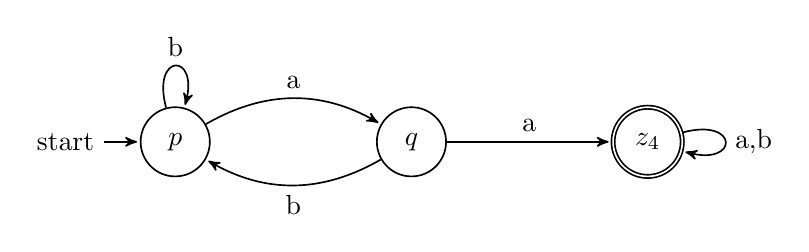
\begin{tikzpicture}[->,>=stealth',shorten >=1pt,auto,node distance=3cm,
										semithick]
	\tikzstyle{every state}=[fill=none,draw=black,text=black]

	\node[initial,state] 						(A)              {$p$};
	\node[state]         						(B) [right of=A] {$q$};
	\node[state, accepting]         (C) [right of=B] {$z_4$};

	\path (A) edge [bend left]	node {a} (B)
						edge [loop above]	node {b} (A)
				(B) edge  						node {a} (C)
						edge [bend left]  node {b} (A)
				(C) edge [loop right] node {a,b} (C);
\end{tikzpicture}

\begin{equation*}
	T(M)=\set{waaw'}{w,w'\in\simpleset{a,b}^\star}
\end{equation*}


\section{CYK-Algorithmus zur Lösung des Wortproblems für Typ-2}\label{algo:cyk}
Mit dem CYK-Algorithmus ist das Wortproblem für Typ-2 in $\mathcal O(n^3)$ entscheidbar.

Hierfür werden alle Ableitungsmöglichkeiten in einer Tabelle geordnet dargestellt. Ist am Ende die Startvariable als Startknoten für die Ableitung möglich, so ist das Wort in $L$.


\subsection*{Am Beispiel:}
Produktionsregeln der Grammatik (CNF):

\begin{equation*}
	S\rightarrow AX|YB, A\rightarrow XA|AB|a, B\rightarrow XY|BB, X\rightarrow YA|a, Y\rightarrow XX|b
\end{equation*}

Eingabewort: $abbaab$

\renewcommand{\arraystretch}{1.2}
\begin{tabular}{ccccccc}
	Länge & a & b & b & a & a & b\\
	\cline{2-7}
	1 & \multicolumn{1}{|c|}{$\simpleset{A,X}$} & \multicolumn{1}{c|}{$\simpleset{Y}$} & \multicolumn{1}{c|}{$\simpleset{Y}$} & \multicolumn{1}{c|}{$\simpleset{A,X}$} & \multicolumn{1}{c|}{$\simpleset{A,X}$} & \multicolumn{1}{c|}{$\simpleset{Y}$}\\
	\cline{2-7}
	2 & \multicolumn{1}{|c|}{$\simpleset{B}$} & \multicolumn{1}{c|}{$\emptyset$} & \multicolumn{1}{c|}{$\simpleset{X}$} & \multicolumn{1}{c|}{$\simpleset{A,S,Y}$} & \multicolumn{1}{c|}{$\simpleset{B}$} &\\
	\cline{2-6}
	3 & \multicolumn{1}{|c|}{$\emptyset$} & \multicolumn{1}{c|}{$\emptyset$} & \multicolumn{1}{c|}{$\simpleset{A,Y,X}$} & \multicolumn{1}{c|}{$\simpleset{A}$} &&\\
	\cline{2-5}
	4 & \multicolumn{1}{|c|}{$\emptyset$} & \multicolumn{1}{c|}{$\simpleset{X}$} & \multicolumn{1}{c|}{$\simpleset{B,X}$} &&&\\
	\cline{2-4}
	5 & \multicolumn{1}{|c|}{$\simpleset{S,Y}$} & \multicolumn{1}{c|}{$\simpleset{B,S}$} &&&&\\
	\cline{2-3}
	6 & \multicolumn{1}{|c|}{$\simpleset{A,B}$} &&&&&\\
	\cline{2-2}
\end{tabular}

Da die unterste Zelle nun $\simpleset{A,B}$ enthält, ist $w=abbaab\not\in L$

\chapter{Anwedungen der Sätze}
\section{Pumping-Lemma für Typ-3}\label{bsp:pumpingLemma}
Für die Sprache $L=\set{a^nb^n}{n\geq 1}$:%
\begin{align*}
	\intertext{Zunächst wählt man ein Wort $x$, mit $|x|\geq n$:}
	x&=a^nb^n \in L,\quad |a^nb^n|=2n>n\\
	\intertext{Nun zu einer beliebigen Zerlegung $x=uvw$, für die die Bedingungen gelten:}
	x&=uvw=a^nb^n\\
	u&=a^{n-l-k} \quad v=a^l \quad w=a^k b^n \text{ mit $l\geq 1$}\\
	x&=(a^{n-l-k}) (a^l) (a^k b^n)\\
	\intertext{Pumpt man nun $v$ mit $v=0$:}
	x&=(a^{n-l-k}) (a^l)^i (a^k b^n)=(a^{n-l-k}) (a^l)^0 (a^k b^n)\\
	x&=(a^{n-l-k}) (a^k b^n) = a^{n-l} b^n \not\in L\text{, da $l\geq 1$}\\
\end{align*}
\section{Myhill-Nerode-Äquivalenz}\label{bsp:myhill}
Für die Sprache $L=\set{w\in\simpleset{a,b}^\star}{w \text{ enthält das Teilwort $abb$}}$:%
\begin{align*}
	\intertext{Finden der Äquivalenzklassen:}
	[\epsilon]&=\simpleset{\epsilon, b, bb, \ldots}\\
	[a]&=\simpleset{a, ba, bba, aba, \ldots}=\set{wa}{w\in\simpleset{a,b}^\star}\\
	[ab]&=\simpleset{ab}=\set{wab}{w\in\simpleset{a,b}^\star}\\
	[abb]&=\simpleset{abb, }=\set{wabbw'}{w,w'\in\simpleset{a,b}^\star}
\end{align*}

\end{document}



\end{document}
